\chapter{东北虎} % Introduction chapter suppressed from the table of contents

中国东北虎是濒危动物,估计国内东北虎数量小于30只,国家动物保护组织做了很多努力。例如,人工饲养。专家尝试把这些人工饲养的东北虎放归野外,但这件事非常不容易。他们能独立在野生环境存活下去吗?下面看看他们遇到的种种困难。\\
首先先选拔了最有潜力的老虎:

\begin{itemize}
\tightlist
\item
  第一次选了一只大体型的年轻老虎,把它放到一个模拟自然环境的大操场由专家观察。开始的时候,老虎还是表现出一般野性老虎的特征,比如小心翼翼地去观察周边的环境,但过了几个小时后,这只老虎顶不住外面的低温环境,还是选择躲回平常的窝里,试验失败。
\item
  另外一只老虎,不怕冷很活跃,但缺乏野生动物的警惕性。比如,习惯了人类,这很容易在野生生活中被害。所以专家也放弃了它。
\end{itemize}

老虎要在野生独立生活,必须自己能找到食物。在自然界,它们最正常的猎物就是鹿,但鹿跑得很快,一小时可以跑五十公里,而且耐力很强。所以专家要看老虎能否捕食到鹿,如果不能,也不能放归野外。在此过程里,专家发现老虎跑步跟觅食的能力都比野生的差很多,太缺少运动。所以专家为他们设计很多运动,比如用汽车拉着轮胎,插上一些鲜肉,引它们奔跑。经过一系列锻炼,它们体力慢慢回到正常,但能不能否捕猎到鹿还是个疑问。一些专家尝试用汽车拖着鹿的尸体奔跑吸引老虎。有些老虎因为平常饲养的时候都没有吃过鹿肉,根本就不感兴趣。剩下两三只老虎追着车,希望抓到鹿,最后有两只年轻老虎赢了。现在就把那些鹿的尸体奖励给获胜的老虎,但发现有那些老虎对着这个鹿的尸体不懂怎么下口。因为以前都是饲养员切好肉给它们吃。最终两只老虎用了好几个小时,慢慢学会怎么可以吃到鹿肉。

我看完这个东北虎纪录片,立马想到一些年轻程序员,他们也一直在保护的环境下工作。例如,他们习惯了管理层或者有经验者对他们没有太多代码质量要求,所以如果要这些年轻程序员注重代码质量,就跟保护区要把饲养的东北虎放回野外一样,得辛辛苦苦培训,才可以提升他们的竞争力。管理层也要了解,如果保护着程序员,对他们写代码的质量没有要求,公司软件产品质量永远不能提升,无法与其它公司竞争。

跟一企业质量官聊,发现越来越多企业开始注重质量,他说:``制定质量流程每家公司都能容易做到,但很多(公司)执行出问题,从我近二十年经验,企业文化很关键,因做好质量的核心是每人都有质量意识,并养成习惯。''

%\href{文件:TigerScreenshot_2022-11-29_082120.jpg}{400px}

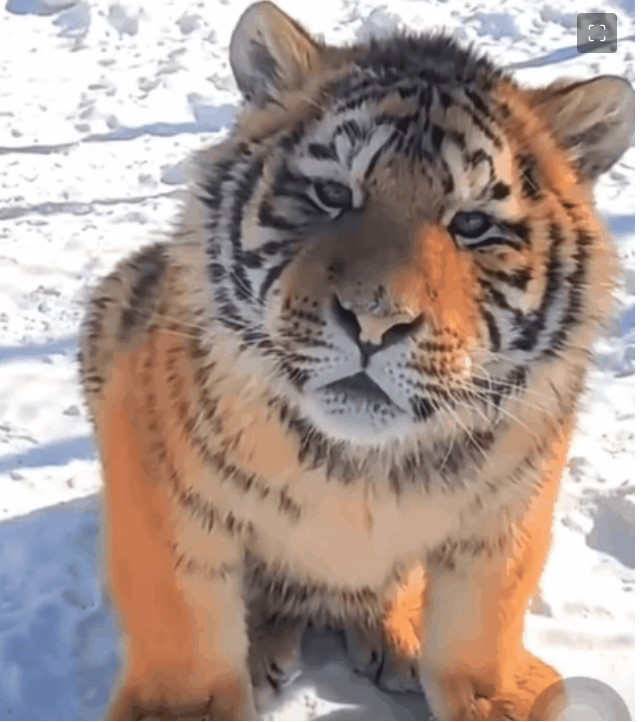
\includegraphics[width=6cm]{TigerScreenshot_2022-11-29_082120.jpg}




